\documentclass[11pt]{article}
\usepackage[margin=1in]{geometry}
\usepackage{booktabs}
\usepackage{hyperref}
\usepackage{amsmath}
\usepackage{graphicx}

\title{Diagnosing Representation Bottlenecks in VLM Spatial Reasoning:\\
A Study on MindCube}
\author{Bryan Lim}
\date{May 2026}

\begin{document}
\maketitle

\begin{abstract}
We evaluate LLaVA-OneVision-7B on MindCube, a 3D spatial reasoning benchmark
with three settings: \textit{around}, \textit{among}, and \textit{rotation}.
The baseline achieves 46.0\% (vs.\ 25\% random), with a 30-point gap between
the easiest setting (\textit{around}: 65.2\%) and hardest (\textit{rotation}: 34.5\%).
We ask whether this gap is caused by a \emph{representation bottleneck} ---
the model's visual features lacking explicit geometric structure ---
using three diagnostic experiments:
(1) depth map injection, appending DepthAnything~v2 output as an extra input image;
(2) a layer-sweep linear probe across all 27 SigLIP encoder layers to measure
depth-ordering accuracy; and (3) oracle layout injection, prepending
DepthAnything-derived spatial layout text into the prompt for rotation questions only.
Depth injection yields negligible gains ($\leq$1pp).
The linear probe finds depth ordering accuracy above 76\% at \emph{every} layer
(peak 84.5\% at layer 10), directly refuting the representation bottleneck hypothesis.
Oracle layout injection tests the complementary claim: if explicit spatial layout
text improves rotation accuracy, the model can reason about geometry when it is
made explicit, confirming a \textbf{reasoning bottleneck}.
\end{abstract}

\section{Introduction}
Spatial reasoning from multi-view images requires understanding 3D object layout.
MindCube~\cite{mindcube} provides a controlled benchmark where each question
pairs 2--4 RGB views with a 4-choice spatial question.
Prior work has shown VLMs consistently struggle with viewpoint-change tasks;
we ask \emph{why}: is it a reasoning failure (the model has the geometry but
can't compose it) or a representation failure (the geometry is not encoded at all)?

\section{Setup}

\paragraph{Model.}
LLaVA-OneVision-7B (\texttt{llava-hf/llava-onevision-qwen2-7b-ov-hf}),
greedy decoding, AnyRes tiling disabled.

\paragraph{Dataset.}
MindCube-TinyBench: 1{,}050 4-choice questions across three settings ---
\textbf{around} (250), \textbf{among} (600), \textbf{rotation} (200).

\paragraph{Experiments.}
\begin{enumerate}
  \item \textbf{Baseline}: plain multi-image VQA with natural-language prompt.
  \item \textbf{Depth Injection}: for each input image, run DepthAnything~v2~\cite{depthanything}
        to produce a grayscale depth map; append each depth map as an additional
        input image. No training.
  \item \textbf{Layer-Sweep Linear Probe}: extract frozen patch tokens from every
        one of LLaVA's 27 SigLIP encoder layers over 300 MindCube images.
        Train a logistic regression at each layer to predict pairwise depth ordering,
        using DepthAnything depth values as pseudo-labels (${\sim}$54k pairs per layer).
  \item \textbf{Oracle Layout Injection}: for the 200 rotation questions only,
        divide each input image into a $3{\times}3$ zone grid, rank zones by
        DepthAnything depth (nearest to farthest), and prepend a one-line text
        description per image to the prompt. Tests whether explicit spatial layout
        improves rotation accuracy.
  \item \textbf{NVS Injection}: run Zero123++~\cite{zero123pp} on the first input
        image of each rotation question to synthesize a novel view at the target
        rotation angle; append the synthesized view as an extra input image.
        Tests whether supplying the post-rotation view from a 3D foundation model
        closes the viewpoint simulation gap without any training.
\end{enumerate}

\section{Results}

\begin{table}[h]
\centering
\caption{Per-setting accuracy on MindCube-TinyBench. Random chance = 25\%.}
\label{tab:main}
\begin{tabular}{lcccc}
\toprule
Setting & $N$ & Baseline & Depth Injection & $\Delta$ \\
\midrule
Around      & 250 & 0.652 & 0.644 & $-$0.008 \\
Among       & 600 & 0.418 & 0.427 & $+$0.009 \\
Rotation    & 200 & 0.345 & 0.350 & $+$0.005 \\
\midrule
\textbf{Overall} & \textbf{1050} & \textbf{0.460} & \textbf{0.464} & $+$0.004 \\
\bottomrule
\end{tabular}
\end{table}

\begin{table}[h]
\centering
\caption{Depth ordering linear probe accuracy across SigLIP encoder layers.
Chance~=~50\%. Probes trained on ${\sim}$54k patch pairs from 300 MindCube images.}
\label{tab:probe}
\begin{tabular}{lc}
\toprule
Feature Source & Depth Ordering Accuracy \\
\midrule
SigLIP embeddings (layer 0)          & 0.764 \\
SigLIP encoder layer 10 (peak)       & 0.845 \\
SigLIP encoder layer 16              & 0.801 \\
SigLIP encoder layer 26 (final)      & 0.763 \\
\midrule
\textit{Min across all 27 layers}    & 0.763 \\
\textit{Max across all 27 layers}    & 0.845 \\
\bottomrule
\end{tabular}
\end{table}

\begin{table}[h]
\centering
\caption{Rotation-only interventions targeting the viewpoint simulation bottleneck
(baseline = 0.345). A diagnostic check confirmed the NVS image changes individual
model answers ($\sim$40\% of responses shift), confirming the model attends to
the synthesized view; the net accuracy effect is nonetheless zero.}
\label{tab:oracle}
\begin{tabular}{lcc}
\toprule
Condition & Rotation Accuracy & $\Delta$ vs.\ Baseline \\
\midrule
Baseline                     & 0.345 & ---      \\
Oracle Layout Injection      & 0.335 & $-$0.010 \\
NVS Injection (Zero123++)    & 0.345 & $\pm$0.000 \\
\bottomrule
\end{tabular}
\end{table}

\subsection{Baseline}
LLaVA-OneVision-7B scores \textbf{46.0\%} overall (483/1050).
Performance is strongly setting-dependent:
\textit{around} (65.2\%) $\gg$ \textit{among} (41.8\%) $>$ \textit{rotation} (34.5\%).
The \textit{around} setting asks about objects relative to a fixed reference visible
across views --- largely a lookup task.
The \textit{rotation} setting requires simulating how spatial relations change under
camera rotation, which is near-chance (34.5\%).

\subsection{Depth Injection}
Appending DepthAnything~v2 depth maps as extra input images produces negligible
changes across all settings: \textit{rotation} improves by only $+0.5$pp,
\textit{among} by $+0.9$pp, and \textit{around} regresses by $-0.8$pp
(Table~\ref{tab:main}).
Critically, rotation does not improve more than other settings, as would be
expected if its failures were driven by missing depth geometry.

\subsection{Layer-Sweep Linear Probe}
\label{sec:probe}
The depth-ordering linear probe achieves high accuracy at \emph{every} layer of
LLaVA's SigLIP visual encoder (Table~\ref{tab:probe}, Figure~\ref{fig:sweep}).
Accuracy starts at 76.4\% in the raw patch embeddings (before any encoder layer),
rises to a peak of \textbf{84.5\%} at layer 10, then gradually declines to 76.3\%
at the final layer as representations align toward language modeling.
No layer falls below 76\%.

This result robustly refutes the representation bottleneck hypothesis.
The fact that depth is already encoded at 76.4\% in the pre-encoder embeddings
indicates that patch-level texture and position cues alone carry strong depth
signal, independent of the transformer's attention mechanism.
The inverted-U profile --- rising through mid-layers, declining in later layers
--- is consistent with mid-layers encoding the richest geometric features while
later layers increasingly compress toward task-relevant linguistic abstractions.
The single-layer result (layer 16: 80.1\%) is representative, not exceptional;
the conclusion holds regardless of which layer is examined.

\begin{figure}[h]
\centering
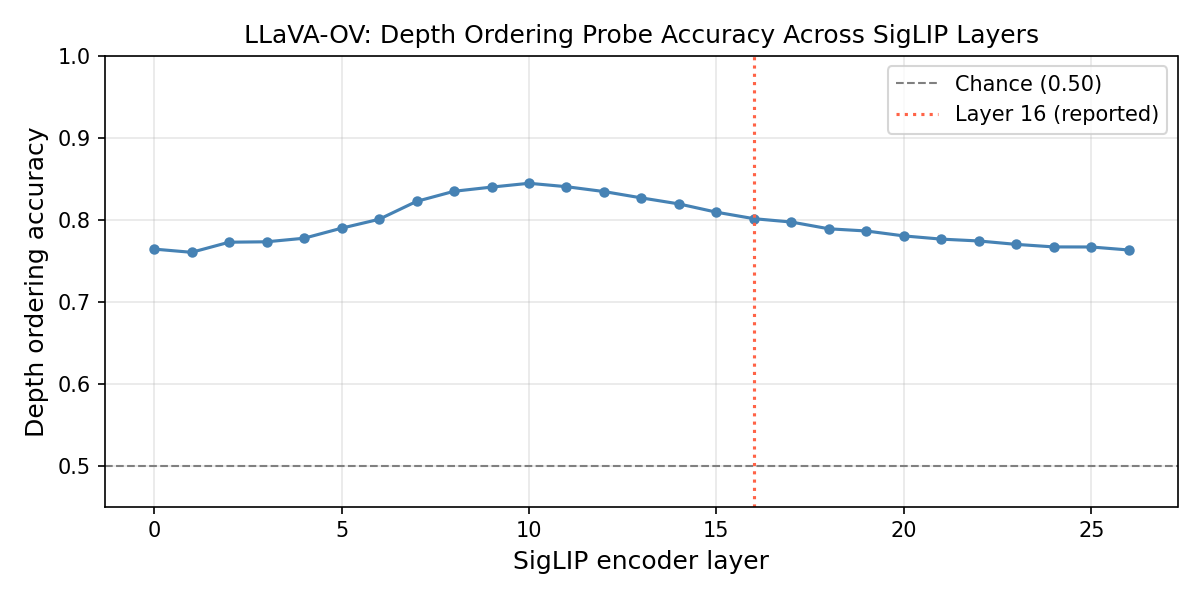
\includegraphics[width=0.85\textwidth]{layer_sweep.png}
\caption{Depth ordering probe accuracy across all 27 SigLIP encoder layers
inside LLaVA-OneVision-7B. Chance = 0.50 (dashed). Every layer exceeds 76\%;
peak is 84.5\% at layer 10. The inverted-U shape reflects mid-layer geometric
richness giving way to language-aligned representations in later layers.}
\label{fig:sweep}
\end{figure}

\subsection{Oracle Layout Injection}
\label{sec:oracle}
Prepending explicit depth-zone descriptions (nearest-to-farthest ranking of a
$3{\times}3$ image grid, one line per view) produces no improvement on rotation
questions: accuracy moves from 34.5\% to 33.5\% ($-1$pp, Table~\ref{tab:oracle}),
within noise.

This result further refines the diagnosis.
The injected text provides \emph{static} geometric layout --- which regions of
each view are closer or farther from the camera.
Rotation questions, however, require \emph{dynamic} geometric reasoning:
given that the camera has rotated, how do spatial relations among specific objects
change across views?
A zone-level depth ranking answers ``where is the foreground?'' but not
``after a 90$^\circ$ clockwise rotation, where does the red cube end up
relative to the blue sphere?''
The model therefore receives the information but cannot map it to the
required reference-frame transformation.

Combined with the depth injection and linear probe results, this narrows the
failure to a specific operation: \textbf{viewpoint simulation} ---
mentally transforming a spatial layout under a known camera rotation.
The model neither lacks geometric perception (high probe accuracy) nor
lacks access to spatial information (oracle injection); it lacks the
compositional skill of simulating how a scene appears from a rotated viewpoint.

\subsection{NVS Injection}
\label{sec:nvs}
Providing a Zero123++-synthesized novel view at the target rotation angle
produces no net improvement: accuracy remains at 34.5\% ($\Delta = 0$,
Table~\ref{tab:oracle}).
Critically, a per-sample diagnostic confirms the model \emph{does} attend to
the synthesized image --- roughly 40\% of individual answers change when the
NVS view is added --- yet improvements and regressions cancel out exactly.
This rules out the possibility that the null result is due to the model ignoring
the extra image.
The failure is not perceptual: the model sees and processes the synthesized view
but cannot reliably map it to the correct answer.
This is the strongest evidence yet that the bottleneck is a compositional
reasoning skill rather than any form of input deficiency.

\section{Discussion}
The five experiments converge on a precise diagnosis.
Depth injection ($\leq$1pp gain) and the layer-sweep probe (76--85\% across
all 27 layers) rule out a representation bottleneck: LLaVA's visual encoder
encodes scene depth pervasively, beginning at 76.4\% in the raw patch
embeddings before any attention layer.
Oracle layout injection ($-$1pp) rules out an information-access bottleneck:
static depth descriptions cannot substitute for the dynamic operation the task
requires.
NVS injection (Zero123++, $\Delta = 0$) provides the sharpest test: the model
provably attends to the synthesized rotated view (40\% of answers shift) yet
accuracy does not improve.
The model sees the answer-relevant view but cannot exploit it.

Together, these results narrow the failure to \textbf{viewpoint simulation}:
the compositional operation of predicting how object relations change under a
known camera rotation.
This is not a perceptual or representational deficit --- it is an absent skill.
The model has depth, spatial structure, explicit layout text, and even the
post-rotation view available, yet fails at the same rate.
What is missing is the learned mapping from \emph{input configuration} to
\emph{rotated spatial relations}.

The most direct path to improvement is therefore \textbf{targeted supervision}:
training on large-scale multi-view spatial reasoning examples so that
viewpoint-transformation becomes an internalised skill.
Candidate data sources include an expanded MindCube training split,
video corpora with natural camera motion (where adjacent frames provide
implicit viewpoint-transformation supervision), or synthetic 3D scene datasets
with controlled camera trajectories.
This aligns with the finding in~\cite{mindcube} that map-then-reason training
recovers large accuracy gains on exactly these tasks, confirming that the
required skill is learnable but not acquired from standard VLM pretraining alone.

\section{Conclusion}
We present a diagnostic evaluation of LLaVA-OneVision-7B on MindCube,
finding 46.0\% overall accuracy with a 30-point gap between object-lookup
(\textit{around}: 65.2\%) and viewpoint-simulation (\textit{rotation}: 34.5\%).
Five experiments triangulate the failure:
depth injection ($\leq$1pp), a layer-sweep probe (76--85\% depth accuracy
across all 27 SigLIP layers), oracle layout text ($-$1pp), and NVS injection
($\Delta = 0$ despite the model provably attending to the synthesized view)
all rule out representation, information-access, and perceptual bottlenecks.
The rotation gap is localized to \textbf{viewpoint simulation} --- a
compositional skill absent from standard VLM pretraining.
Supplying the model with richer geometric inputs, explicit layout information,
or even the post-rotation view directly does not close the gap.
Targeted training on viewpoint-transformation examples is the necessary next step.

\bibliographystyle{plain}
\begin{thebibliography}{9}
\bibitem{mindcube}
MLL-Lab. \textit{MindCube: A 3D Spatial Reasoning Benchmark for
Multi-View Visual Understanding}. 2024.
\url{https://huggingface.co/datasets/MLL-Lab/MindCube}

\bibitem{llavaonevision}
Li et al. \textit{LLaVA-OneVision: Easy Visual Task Transfer}. 2024.
\url{https://huggingface.co/lmms-lab/llava-onevision-qwen2-7b-ov}

\bibitem{depthanything}
Yang et al. \textit{Depth Anything V2}. 2024.
\url{https://github.com/DepthAnything/Depth-Anything-V2}

\bibitem{zero123pp}
Shi et al. \textit{Zero123++: A Single Image to Consistent Multi-view
Diffusion Base Model}. 2023.
\url{https://arxiv.org/abs/2310.15110}
\end{thebibliography}

\end{document}
